\chapter{Auswertung}
Zur Bestimmung der Geschwindigkeit des Lichtes ist zu beachten, dass der Strahl die Strecke \(s\) auf dem Hin- und auf
dem Rückweg jeweils ein mal durchläuft. Die Streckenänderung \(\Delta s\) geht also mit einem Faktor 2 in die Berechnung
ein.
%
%=================================================================
%
\section{Lichtgeschwindigkeit}
Werden die im Versuch gemessenen Werte für die Laufzeitdifferenz \(\Delta t\) über den Strahlweg \(s\) des Messsignals aufgetragen,
so kann die Steigung der Ausgleichsgeraden als Kehrwert der Lichtgeschwindigkeit in \(\frac{m}{ns}\) interpretiert werden.
\begin{figure}[h]
    \centering
    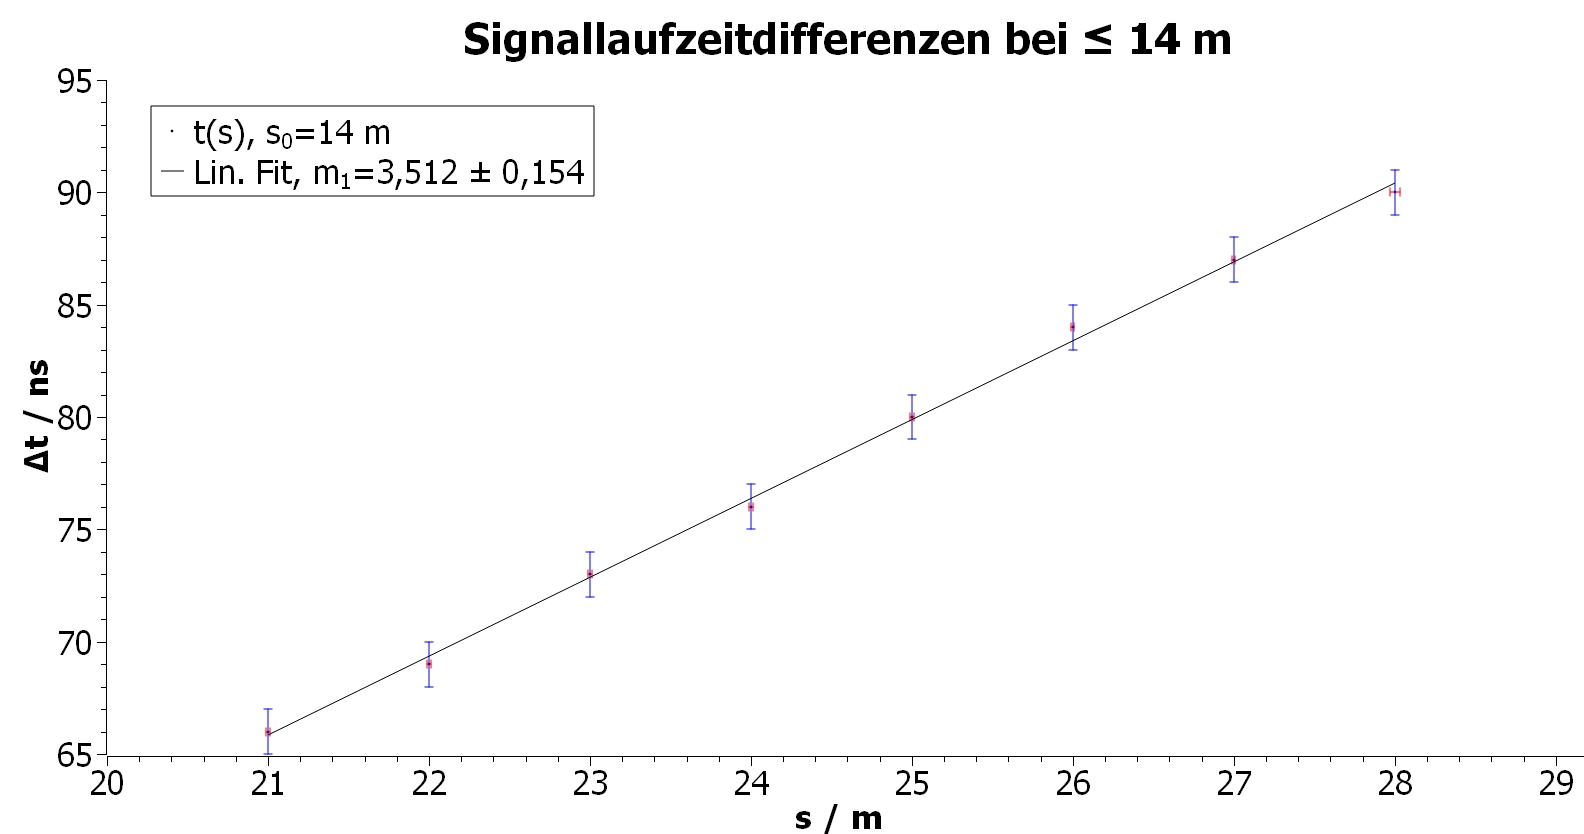
\includegraphics[width=.9\textwidth]{scidavis/14m.jpeg}
    \caption[Signallaufzeitunterschiede mit \(s_0 = \SI{14}{m}\)]{\(\Delta t(s)\)-Diagram im Intervall \( \SI{10,5}{m} \leq s \leq \SI{14}{m}\) mit \(s_0=\SI{14}{m}\).}
    \label{fig:14m}
\end{figure}
%
\begin{figure}[h]
    \centering
    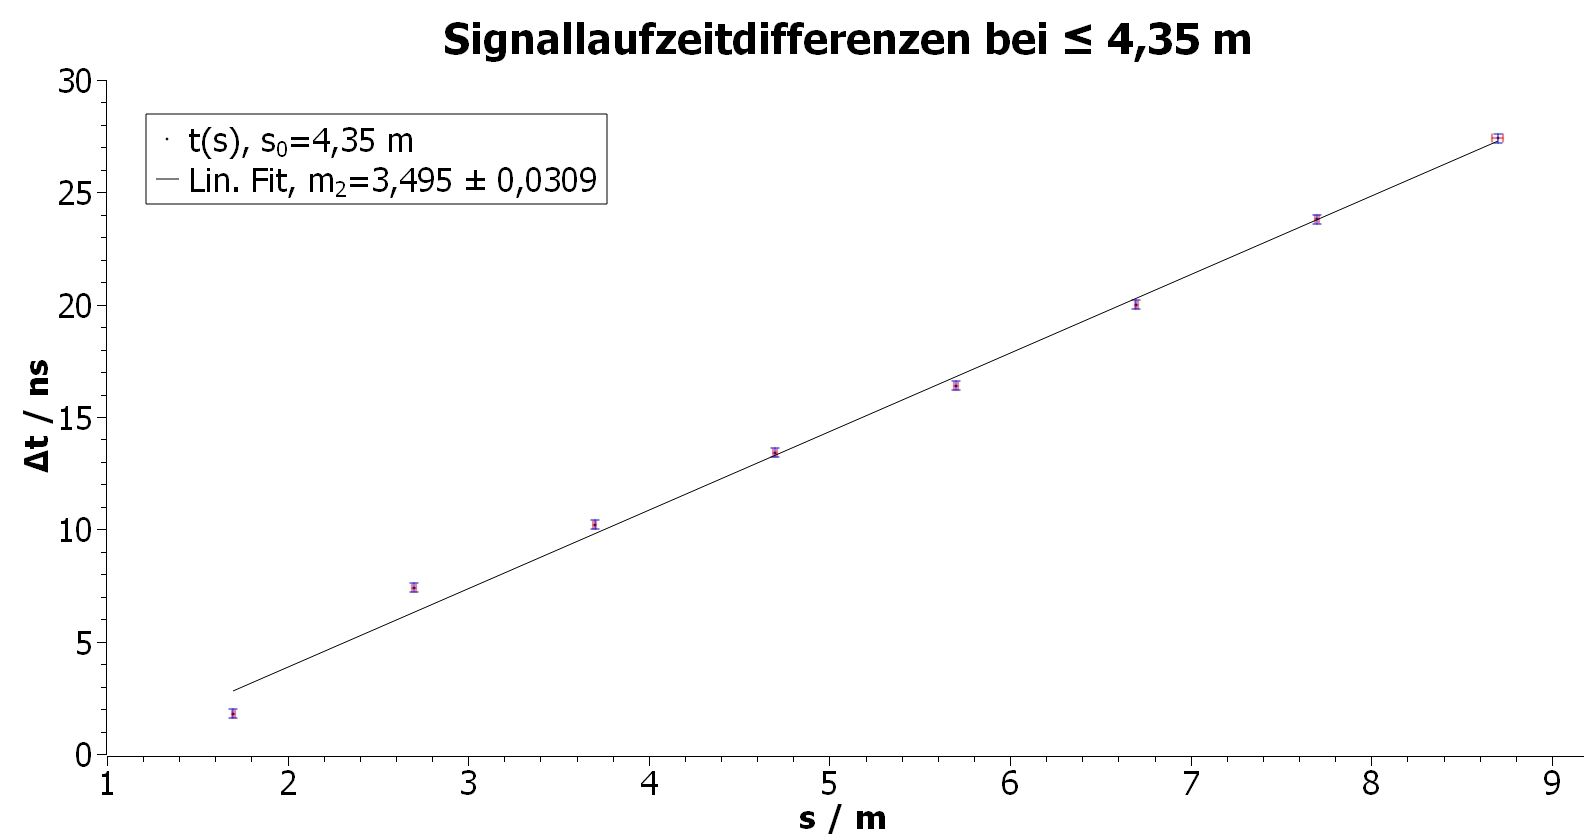
\includegraphics[width=.9\textwidth]{scidavis/4.35m.jpeg}
    \caption[Signallaufzeitunterschiede mit \(s_0 = \SI{4,35}{m}\)]{\(\Delta t(s)\)-Diagram im Intervall \( \SI{0,85}{m} \leq s \leq \SI{4,35}{m}\) mit \(s_0=\SI{4,35}{m}\).}
    \label{fig:4.35m}
\end{figure}
%
\bild{fig:14m} zeigt die Messung bei einer Anfangsdistanz des Prismen-Reflektors zur Strahlquelle von \SI{14}{m} unter einer Reduktion
der Distanz in Schritten von \SI{0,5}{m} bis herunter zu \SI{10,5}{m}. \bild{fig:4.35m} entsprechend die Messung bei einer
Anfangsdistanz von \SI{4,35}{m} herunter zu \SI{0,85}{m} bei gleicher Schrittweite. Prakmatische Limitierungen der
Versuchsumgebung - eine \glqq{}Lücke\grqq{} zwischen den Labortischen - ließen keine kontinuierliche Messungen im Bereich
zwischen \(\SI{10,5}{m} \text{ und } \SI{4,35}{m}\) zu.\par
Die Steigung der Ausgleichsgeraden \(m_{1,2}\) der Diagramme in \bild{fig:14m} und \bild{fig:4.35m} kann als Inverse der
Lichtgeschwindigkeit mit
\begin{equation}
    m = \frac{\Delta t}{\Delta s} = c^{-1} \quad \Leftrightarrow \quad c = m^{-1}
    \label{eq:lightspeed}
\end{equation}
verstanden werden.\par
Die beiden Messreihen führen so zu Werten für die Lichtgeschwindigkeit in Luft von
\begin{equation}
    m_1^{-1} = c_1 = \left( \SI{3,512}{\frac{ns}{m}} \right)^{-1} = \SI{2,847 \cdot 10^8}{\frac{m}{s}}
\end{equation}
und
\begin{equation}
    m_2^{-1} = c_2 = \left( \SI{3,495}{\frac{ns}{m}} \right)^{-1} = \SI{2,861 \cdot 10^8}{\frac{m}{s}}
\end{equation}
%
\section{Brennweite der \textsc{Fresnel}-Linse}
Die Brennweite kann durch die Gegenstands- und Bildweite bestimmt werden. Gemessen wurde für die Gegenstandsweite $ g=(485\pm 5)\SI{}{mm} $ und für die Bildweite $ b=(470\pm 5)\SI{}{mm} $.\\
Nach \gl{eq:brenn} kann die Brennweite $ f $ wie folgt berechnet werden:
\begin{align}
    f = \left( \frac{1}{b} + \frac{1}{g} \right)^{-1} = \left( \frac{1}{\SI{470}{mm}} + \frac{1}{\SI{485}{mm}} \right)^{-1} = \SI{238,7}{mm}
    \label{eq:brenn_val}
\end{align}
Der rechnerische Wert für die Brennwete weicht um \((136,3 \pm 2,5)\SI{}{mm}\) oder \((36,3 \pm 0,6)\%\) von der Angabe des Herstellers $ f_{H}=\SI{375}{mm} $ ab.
%
\section{Abweichung der Lichtgeschwindigkeit}
Die Abweichungen der Lichtgeschwindigkeiten sind durch die Fehlerfortpflanzung der Steigungen folgendermaßen zu bestimmen:
\begin{align}
    \Delta c_{1}    &= \left\vert \frac{\partial c_{1}}{\partial m_{1}} \right\vert \cdot \Delta m_{1} = m_{1}^{-2} \cdot \Delta m_{1} \nonumber \\
                    &= \left( 3,512 \cdot 10^{-9} \SI{}{\frac{s}{m}} \right)^{-2} \cdot 0,154\cdot 10^{-9} \SI{}{\frac{s}{m}} \nonumber \\
                    &= 0,125\cdot 10^{8} \SI{}{\frac{m}{s}}
\end{align}
\begin{align}
    \Delta c_{2}    &= \left\vert \frac{\partial c_{2}}{\partial m_{2}} \right\vert \cdot \Delta m_{2} = m_{2}^{-2} \cdot \Delta m_{2} \nonumber \\
                    &= \left(3,495\cdot 10^{-9}\SI{}{\frac{s}{m}}\right)^{-2} \cdot 0,0309 \cdot 10^{-9} \SI{}{\frac{s}{m}} \nonumber \\
                    &= 0,025\cdot 10^{8} \SI{}{\frac{m}{s}}
\end{align}
Für die Lichtgeschwindigkeiten ergibt sich also:
\begin{align}
    c_{1} &= (2,85 \pm 0,13)\cdot 10^{8}\SI{}{\frac{m}{s}}\\
    c_{2} &= (2,86 \pm 0,03)\cdot 10^{8}\SI{}{\frac{m}{s}}
\end{align}
%
\section{Abweichung der Brennweite}
Der Fehler der Brennweite ist abhängig von den Abweichungen der Gegenstands- und Bildweite:
\begin{align}
    \Delta f    &= \left\vert \frac{\partial f}{\partial b} \right\vert \cdot \Delta b + \left\vert \frac{\partial f}{\partial g} \right\vert \cdot \Delta g = \frac{1}{b^{2}} \cdot \left(\frac{1}{b}+\frac{1}{g} \right)^{-2} \cdot \Delta b + \frac{1}{g^{2}} \cdot \left(\frac{1}{b}+\frac{1}{g} \right)^{-2} \cdot \Delta g \nonumber \\
                &= \frac{1}{(\SI{470}{mm})^{2}} \cdot \left(\frac{1}{\SI{470}{mm}}+\frac{1}{\SI{485}{mm}} \right)^{-2} \cdot \SI{5}{mm} + \frac{1}{(\SI{485}{mm})^{2}} \cdot \left(\frac{1}{\SI{470}{mm}}+\frac{1}{\SI{485}{mm}} \right)^{-2} \cdot \SI{5}{mm} \nonumber \\
                &=\SI{1,29}{mm}+\SI{1,21}{mm} \nonumber \\
                &=\SI{2,50}{mm}
\end{align}
Die ermittelte Brennweite ist demnach:
\begin{equation}
    f=(238,7 \pm 2,5)\SI{}{mm}
\end{equation}